\documentclass[a4 paper]{article}
\usepackage[inner=2.0cm,outer=2.0cm,top=2.5cm,bottom=2.5cm]{geometry}
\usepackage{setspace}
\usepackage[rgb]{xcolor}
\usepackage{verbatim}
\usepackage{subcaption}
\usepackage{amsgen,amsmath,amstext,amsbsy,amsopn,tikz,amssymb}
\usepackage{fancyhdr}
\usepackage[colorlinks=true, urlcolor=blue,  linkcolor=blue, citecolor=blue]{hyperref}
\usepackage[colorinlistoftodos]{todonotes}
\usepackage{rotating}
\usepackage{booktabs}
\newcommand{\ra}[1]{\renewcommand{\arraystretch}{#1}}

\newtheorem{thm}{Theorem}[section]
\newtheorem{prop}[thm]{Proposition}
\newtheorem{lem}[thm]{Lemma}
\newtheorem{cor}[thm]{Corollary}
\newtheorem{defn}[thm]{Definition}
\newtheorem{rem}[thm]{Remark}
\numberwithin{equation}{section}

\newcommand{\homework}[6]{
   \pagestyle{myheadings}
   \thispagestyle{plain}
   \newpage
   \setcounter{page}{1}
   \noindent
   \begin{center}
   \framebox{
      \vbox{\vspace{2mm}
    \hbox to 6.28in { {\bf CSE 211:~Discrete Mathematics \hfill {\small (#2)}} }
       \vspace{6mm}
       \hbox to 6.28in { {\Large \hfill #1  \hfill} }
       \vspace{6mm}
       \hbox to 6.28in { {\it Instructor: {\rm #3} \hfill  {\rm #5} \hfill  {\rm #6}} \hfill}
       \hbox to 6.28in { {\it Assistant: #4  \hfill #6}}
      \vspace{2mm}}
   }
   \end{center}
   \markboth{#5 -- #1}{#5 -- #1}
   \vspace*{4mm}
}

\newcommand{\problem}[2]{~\\\fbox{\textbf{Problem #1}}\hfill (#2 points)\newline\newline}
\newcommand{\subproblem}[1]{~\newline\textbf{(#1)}}
\newcommand{\D}{\mathcal{D}}
\newcommand{\Hy}{\mathcal{H}}
\newcommand{\VS}{\textrm{VS}}
\newcommand{\solution}{~\newline\textbf{\textit{(Solution)}} }

\newcommand{\bbF}{\mathbb{F}}
\newcommand{\bbX}{\mathbb{X}}
\newcommand{\bI}{\mathbf{I}}
\newcommand{\bX}{\mathbf{X}}
\newcommand{\bY}{\mathbf{Y}}
\newcommand{\bepsilon}{\boldsymbol{\epsilon}}
\newcommand{\balpha}{\boldsymbol{\alpha}}
\newcommand{\bbeta}{\boldsymbol{\beta}}
\newcommand{\0}{\mathbf{0}}


\begin{document}
\homework{Homework \#1}{Due: 17/11/20}{Dr. Zafeirakis Zafeirakopoulos}{Gizem S\"ung\"u}{}{}
\textbf{Course Policy}: Read all the instructions below carefully before you start working on the assignment, and before you make a submission.
\begin{itemize}
\item It is not a group homework. Do not share your answers to anyone in any circumstance. Any cheating means at least -100 for both sides. 
\item Do not take any information from Internet.
\item No late homework will be accepted. 
\item For any questions about the homework, send an email to gizemsungu@gtu.edu.tr
\item The homeworks (both latex and pdf files in a zip file) will be
submitted into the course page of Moodle.
\item The latex, pdf and zip files of the homeworks should be saved as
"Name\_Surname\_StudentId".$\{$tex, pdf, zip$\}$.
\item If the answers of the homeworks have only calculations without any formula or any explanation -when needed- will get zero.
\item Writing the homeworks on Latex is strongly suggested. However, hand-written paper is still accepted $\textbf{IFF}$ hand writing of the student is clear and understandable to read, and the paper is well-organized. Otherwise, the assistant cannot grade the student's homework.
\end{itemize}

\problem{1: Conditional Statements}{5+5+5=15}
State the converse, contrapositive, and inverse of each of these conditional statements.


\subproblem{a} If it snows tonight, then I will stay at home.
\solution
%%%%%%REMOVE \newline commands while writing your answer%%%%%
\newline
\newline
\textbf{Converse:} If I stay at home then it will snow
\newline
\newline
\textbf{Contrapositive:} If I will not stay at home then it will not snot
\newline
\newline
\textbf{Inverse:} If it doesn't snow tonight then I will not stay at home
\newline




\subproblem{b} I go to the beach whenever it is a sunny summer day.
\solution
%%%%%%REMOVE \newline commands while writing your answer%%%%%
\newline
\newline
\textbf{Converse:} If I go to the beach then it is a sunny summer day
\newline
\newline
\textbf{Contrapositive:} If I don't go to the beach then it is not a sunny summer day
\newline
\newline
\textbf{Inverse:} If it isn't a sunny summer day then I don't go to the beach
\newline
\newline
\newline
\newline
\newline


\subproblem{c} If I stay up late, then I sleep until
noon.
\solution
%%%%%%REMOVE \newline commands while writing your answer%%%%%
\newline
\newline
\textbf{Converse:} If I sleep until noon then I will stay up late
\newline
\newline
\textbf{Contrapositive:} If I don't sleep until noon then I will not stay up late
\newline
\newline
\textbf{Inverse:} If I don't stay up late then I don't sleep until noon
\newline
\newline


\problem{2: Truth Tables For Logic Operators}{5+5+5=15}
Construct a truth table for each of the following compound propositions.
\subproblem{a} (p $\oplus$ $\neg$ q)
\solution

\begin{table1}
\centering
\begin{tabular}{|l|l|l|l|} 
\hline
p & q & $\neg$q & (p $\oplus$ $\neg$ q)  \\ 
\hline
1 & 1 & 0 & 1  \\ 
\hline
1 & 0 & 1 & 0  \\ 
\hline
0 & 1 & 0 & 0  \\ 
\hline
0 & 0 & 1 & 1  \\
\hline
\end{tabular}
\end{table1}

\subproblem{b} (p $\iff$ q) $\oplus$ ( $\neg$ p $\iff$ $\neg$ r)
\solution 

\begin{table2}
\centering
\begin{tabular}{|l|l|l|l|l|l|l|l|} 
\hline
p & q & r & $\neg$p & $\neg$r & p $\iff$ q & $\neg$p $\iff$ $\neg$q & (p $\iff$ q) $\oplus$ ( $\neg$ p $\iff$ $\neg$ r)  \\ 
\hline
1 & 1 & 1 & 0 & 0 & 1 & 1 & 0  \\ 
\hline
1 & 1 & 0 & 0 & 1 & 1 & 0 & 1  \\ 
\hline
1 & 0 & 1 & 0 & 0 & 0 & 1 & 1  \\ 
\hline
0 & 1 & 1 & 1 & 0 & 0 & 0 & 0  \\ 
\hline
1 & 0 & 0 & 0 & 1 & 0 & 0 & 0  \\ 
\hline
0 & 1 & 0 & 1 & 1 & 0 & 1 & 1  \\ 
\hline
0 & 0 & 1 & 1 & 0 & 1 & 0 & 1  \\ 
\hline
0 & 0 & 0 & 1 & 1 & 1 & 1 & 0  \\
\hline
\end{tabular}
\end{table2}


\subproblem{c} (p $\oplus$ q) $\Rightarrow$ (p $\oplus$ $\neg$ q)
\solution

\begin{table3}
\centering
\begin{tabular}{|l|l|l|l|l|l|} 
\hline
p & q & $\neg$q & (p $\oplus$ q) & (p $\oplus$ $\neg$ q) & (p $\oplus$ q) $\Rightarrow$ (p $\oplus$ $\neg$ q)  \\ 
\hline
1 & 1 & 0 & 0 & 1 & 1  \\ 
\hline
1 & 0 & 1 & 1 & 0 & 0  \\ 
\hline
0 & 1 & 0 & 1 & 0 & 0  \\ 
\hline
0 & 0 & 1 & 0 & 1 & 1  \\
\hline
\end{tabular}
\end{table3}

\newpage


\problem{3: Predicates and Quantifiers}{21}
There are three predicate logic statements which represent English sentences as follows.

\begin{itemize}
	\item P(x): "x can speak English."
	\item Q(x): "x knows Python."
	\item H(x): "x is happy."
\end{itemize}

Express each of the following sentences in terms of P(x), Q(x), H(x), quantifiers, and logical connectives or vice versa. The domain
for quantifiers consists of all students at the university.

\subproblem{a} There is a student at the university who can speak English and who knows Python.
\solution
\newline

$\exists x (P(x) \wedge Q(x))$

\newline

\subproblem{b} There is a student at the university who can speak English but who doesn’t know Python.
\solution
\newline

$\exists x (P(x) \wedge \neg Q(x))$

\subproblem{c} Every student at the university either can speak English or knows Python.
\solution
\newline

$\forall x (P(x) \oplus Q(x))$


\newline

\subproblem{d} No student at the university can speak English or knows Python.
\solution
\newline

$\neg \exists x ( P(x) \vee Q(x))$

\newline


\subproblem{e} If there is a student at the university who can speak English and know Python, then she/he is happy.
\solution
\newline

$\forall x ( (P(x) \wedge Q(x) ) \Rightarrow H(x)) $


\newline
\subproblem{f} At least two students are happy.
\solution
\newline

$\exists x H(x)$

\newline
\subproblem{g} $\neg \forall x (Q(x) \wedge P(x))$
\solution
\newline
Not every student know Python and can speak English
\newline

\problem{4: Mathematical Induction}{21}
Prove that 3 + 3 . 5 + 3 . $5^2$ + . . . + 3 . $5^n$ =$\frac{3(5^{n+1} - 1)}{4}$
whenever n is a nonnegative integer.
\solution

for n = 0  \hspace{2.5cm} 3 = $\frac{3\times(5-1)}{4}$  $\Rightarrow$ 3 = 3
\newline
\newline

for n = k  \hspace{2.5cm} $3 + 3\times5 + \cdots + 3\times5^k + 3\times5^{k+1} = \frac{3\times(5^{k+1}-1)}{4}$ \\
\newline

for n = k+1  \hspace{2.5cm} $3 + 3\times5 + \cdots + 3\times5^{k+1} + 3\times5^{k+2} = \frac{3\times(5^{k+2}-1)}{4}$ \\

\newline

If we subtract the second equation from the third equation, we get: \\

$ 3\times5^{k+1}  =  \frac{3 \times (5^{k+2}-1) - 3\times(5^{k+1}-1)}{4}$ \\

\newline

$ 3\times5^{k+1}  =  \frac{3 \times 5^{k+2} - 3\times5^{k+1} - 3 + 3}{4}$ \\

\newline

$ 3\times5^{k+1}  =  \frac{3 \times 5^{k+1} \times (5-1) }{4}$ \\

\newline

$ 3\times5^{k+1}  =  3\times5^{k+1} $ \\


\problem{5: Mathematical Induction}{20}
Prove that $n^2$ - 1 is divisible by 8 whenever n is an odd
positive integer.
\solution
\newline

for n = 1 \hspace{2.5cm} $1^1 - 1 = 0$ (it is divisible by 8) \\
\newline

for n = 2k+1 \hspace{2.5cm} $(2 \times (k+1)^2) -1 = 2\times (k+1) \times (k)$ \\
\newline

for n = 2k+3 \hspace{2.5cm} $(2 \times (k+3)^2) -1 = (2\times k + 4 ) \times (2\times k + 2) $ \\

$ =  4\times k^2 + 12\times k + 8 $ \\
\newline
for any integer of x \\
\newline
$ =  4 \times (k^2 + 3\times k + 2) = 4 \times (k+2)(k+1) = 8 \times x$ \\
\newline

$ = (k+2)(k+1) = 2 \times x $ \\
\newline

It is guarantee that an expression like k+2 times k+1 is divisible by 2





\newline
\problem{6: Sets}{8}
Which of the following sets are equal? Show your work step by step.\newline
\subproblem{a} $\{$t : t is a root of $x^2$ – 6x + 8 = 0$\}$
\newline
\newline
$ a = \{2,4\}$
\newline
\subproblem{b} $\{$y : y is a real number in the closed interval [2, 3]$\}$
\newline
\newline
$ b = [2,3]$
\newline
\subproblem{c} $\{$4, 2, 5, 4$\}$
\newline
\newline
$ c = \{2,4,5\}$
\newline
\subproblem{d} $\{$4, 5, 7, 2$\}$ - $\{$5, 7$\}$
\newline
\newline
$ d = \{2,4\}$
\newline
\subproblem{e} $\{$q: q is either the number of sides of a rectangle or the number of digits in any integer between 11 and 99$\}$\\
\newline
\newline
$ e = \{2\} \vee \{3\}$
\newline
\solution

We can find elements of the set a by delta \\

$\Delta = b^2 - 4ac$ \\
$x1,2 = \frac{-b +- \sqrt{\Delta}}{2\times a}$ \\

The set a and the set d are equal

\newpage
\problem{Bonus: Logic in Algorithms}{20}

Let p and q be the statements as follows.

\begin{itemize}
	\item $\textbf{p:}$ It is sunny.
	\item $\textbf{q:}$ The flowers are blooming.
\end{itemize}

\begin{figure*}[htp]
	\centering
	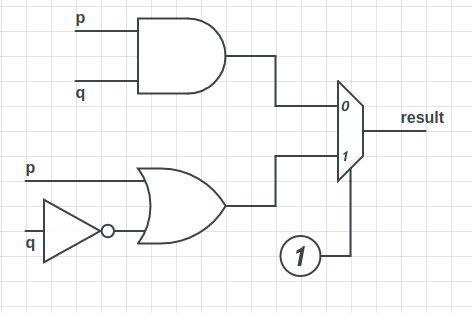
\includegraphics[scale=0.5]{circuit.png}
	\caption{Combinational Circuit}
	\label{fig: circuit}
	
\end{figure*}

In Figure \ref{fig: circuit}, the two statements are used as input. The circuit has 3 gates as AND, OR and NOT operators. It has also a 2x1 multiplexer\footnote{https://www.geeksforgeeks.org/multiplexers-in-digital-logic/} which provides to select one of the two options. 
\subproblem{a} Write the sentence that "result" output has.
\solution
\newline
\subproblem{b} Convert Figure \ref{fig: circuit} to an algorithm which you can write in any programming language that you prefer (including pseudocode).
\solution

\end{document} 
